\documentclass[a4paper, 11pt]{article}
\usepackage{comment}
\usepackage{lipsum} 
\usepackage{fullpage} %cambiar margen
\usepackage[a4paper, total={7in, 10in}]{geometry}

\usepackage{amssymb,amsthm} 
\usepackage{amsmath}
\newtheorem{theorem}{Theorem}
\newtheorem{corollary}{Corollary}
\usepackage{graphicx}
\usepackage{tikz}
\usetikzlibrary{arrows}
\usepackage{verbatim}
%\usepackage[numbered]{mcode}
\usepackage{float}
\usepackage{tikz}
\usetikzlibrary{shapes,arrows}
\usetikzlibrary{arrows,calc,positioning}
\usepackage{mathpazo} %tipo de letra 
\usepackage[utf8]{inputenc} %codificación
\usepackage[T1]{fontenc} %digitación de tildes y ñ
\usepackage[spanish]{babel} %paquete de soporte español

\tikzset{
	block/.style = {draw, rectangle,
		minimum height=1cm,
		minimum width=1.5cm},
	input/.style = {coordinate,node distance=1cm},
	output/.style = {coordinate,node distance=4cm},
	arrow/.style={draw, -latex,node distance=2cm},
	pinstyle/.style = {pin edge={latex-, black,node distance=2cm}},
	sum/.style = {draw, circle, node distance=1cm},
}
\usepackage{xcolor}
\usepackage{mdframed}
\usepackage[shortlabels]{enumitem}
\usepackage{indentfirst}
\usepackage{hyperref}

\usepackage{listings}
\lstset{literate=
  {á}{{\'a}}1
  {é}{{\'e}}1
  {í}{{\'i}}1
  {ó}{{\'o}}1
  {ú}{{\'u}}1
  {Á}{{\'A}}1
  {É}{{\'E}}1
  {Í}{{\'I}}1
  {Ó}{{\'O}}1
  {Ú}{{\'U}}1
  {ñ}{{\~n}}1
  {ü}{{\"u}}1
  {Ü}{{\"U}}1
}

\lstdefinestyle{customc}{
  belowcaptionskip=1\baselineskip,
  breaklines=true,
  frame=L,
  xleftmargin=\parindent,
  language=Python,
  showstringspaces=false,
  basicstyle=\footnotesize\ttfamily,
  keywordstyle=\bfseries\color{green!40!black},
  commentstyle=\itshape\color{purple!40!black},
  identifierstyle=\color{blue},
  stringstyle=\color{orange},
}

\lstdefinestyle{customasm}{
  belowcaptionskip=1\baselineskip,
  frame=L,
  xleftmargin=\parindent,
  language=[x86masm]Assembler,
  basicstyle=\footnotesize\ttfamily,
  commentstyle=\itshape\color{purple!40!black},
}

\lstset{escapechar=@,style=customc}



\renewcommand{\thesubsection}{\thesection.\alph{subsection}}

\newenvironment{problem}[2][Ejercicio]
{ \begin{mdframed}[backgroundcolor= red!50] \textbf{#1 #2} \\}
	{  \end{mdframed}}

% Define solution environment
\newenvironment{solution}
{\textcolor{blue}{\textbf{\textit{Solución:\\\noindent}}}}


\renewcommand{\qed}{\quad\qedsymbol}

% \\	
\begin{document}
	\noindent
	%%%%%%%%%%%%%%%%%%%%%%%%%%%%%%%%%%%%
	
	\begin{minipage}[b][1.2cm][t]{0.8\textwidth}
		\large\textbf{César Isaí García Cornejo} \hfill \textbf{Tarea 2}  \\
		cesar.cornejo@cimat.mx \hfill \\
		\normalsize Estadística Bayesiana \hfill Semestre 4\\
	\end{minipage}
	
	\hspace{14.4cm}
	\begin{minipage}[b][0.03cm][t]{0.12\linewidth}
		
		\vspace{-2.2cm}
		%%%La Ruta dependerá de donde este alojado el main y la imagen
		
\includegraphics[scale=0.3]{Figures/EscudoCimat.png}
	\end{minipage}
	
	\noindent\rule{7in}{2.8pt}
	
	%%%%%%%%%%%%%%%%%%%%%
	%%%%%%%%%%%%%%%%%%%%%%%%%%%%%%%%%%%%%%%%%%%%%%%%%%%%%%%%%%%%%%%%%%%%%%%%%%%%%%%%%%%%%%%%%%%%%%%%%%%%%%%%%%%%%%%%%%%
	% Problem 1
	%%%%%%%%%%%%%%%%%%%%%%%%%%%%%%%%%%%%%%%%%%%%%%%%%%%%%%%%%%%%%%%%%%%%%%%%%%%%%%%%%%%%%%%%%%%%%%%%%%%%%%%%%%%%%%%%%%%%%%%%%%%%%%%%%%%%%%%%
	\setlength{\parskip}{\medskipamount}
	\setlength{\parindent}{0pt}
%/////////// Ejercicio 1 /////////////////
\begin{problem}{1} 
    Suponga que $X_i \sim U(0,\theta)$ independientes. ¿Cómo haría inferencia bayesiana (conjugada) sobre $\theta$ para analizar la Hipótesis $H_0: \theta < 20$ vs $H_1: \theta \geq 20$? Ejemplo: Tenemos un equipo electrónico cuya confiabilidad se puede describir con una distribución uniforme. Los tiempos de falla en meses de 30 de estos aparatos son: 7.7, 1.2, 5.5, 5.5, 13.0, 12.0, 9.7, 11.0, 18.0, 19.0, 16.0, 9.3, 6.8, 3.7, 4.8, 6.1, 2.2, 3.6, 9.9, 8.0, 19.0, 11.0, 15.0, 8.1, 15.0, 5.1, 12.0, 7.3, 2.1, 14.0. ¿Qué se puede concluir entonces del contraste de hipótesis anterior?    
\end{problem}

\begin{solution} 
    Dado que se nos pide hacer una análisis conjugado para un modelo donde $X_i \sim U(0,\theta)$ entonces es que se tiene que proponer una distribución a priori $\theta \sim Pareto(\alpha_0,\beta_0)$. Mostraremos que en efecto estamos ante un análisis conjugado. Primeramente, recordemos que la densidad de una distribución $Pareto(\alpha,\beta)$ es
    \begin{align}
        f(x) = \alpha \beta ^\alpha x^{-(\alpha +1)} \mathbb{1}_{[\beta,\infty)}(x).
        \label{Pareto}
    \end{align}
    Notemos que el soporte de la distribución Pareto depende del parámetro $\beta$.

    Por otro lado, la distribución posterior del parámetro $\theta$ es
    \begin{align}
        f(\theta|X^n) \propto f(\theta) \mathcal{L}(\theta),
    \end{align}
    con la distribución a priori $\theta \sim Pareto(\alpha_0,\beta_0)$ se sigue que
    \begin{align*}
        f(\theta|X^n) \propto \alpha_0 \beta_0^{\alpha_0} \theta^{-(\alpha_0 +1)} \mathbb{1}_{[\beta_0,\infty)}(\theta) \prod_{i = 1}^{n} \frac{1}{\theta} \mathbb{1}_{[0,\theta]}(X_i).
    \end{align*}
    Observemos que la verosimilitud se anula si existe un $i$ tal que $X_i > \theta$. Entonces, para tener verosimilitud no nula se requiere que para todo $i$ se cumpla $\theta \geq X_i$. Dicho de otra forma, basta con que se cumpla que $\theta \geq X_{(n)}$ donde $X_{(n)} = max_{i}\{X_i\}$ también conocida como la estadística de orden superior. Por tanto,
    \begin{align*}
        f(\theta|X^n) \propto \theta^{-(\alpha_0 + n +1)} \mathbb{1}_{[\beta_0,\infty)}(\theta) \mathbb{1}_{[X_{(n)}, \infty)}(\theta).
    \end{align*}
    Recordemos que el producto de dos funciones indicadores sobre dos conjuntos es la función indicadora de la intersección. Así
    \begin{align}
        f(\theta|X^n) \propto \theta^{-(\alpha_0 + n +1 )} \mathbb{1}_{[\max\{X_{(n)}, \beta_0\}, \infty)} (\theta).
        \label{1.03}
    \end{align}
    Contrastando (\ref{1.03}) con (\ref{Pareto}) que es el kernel de una distribución Pareto, lo que muestra que en efecto son familias conjugadas. 
    
    Por tanto, la distribución posterior es también una distribución Pareto
    \begin{align}
        \theta|X^n \sim Pareto(\alpha_p, \beta_p),
    \end{align}
    donde $\alpha_p = \alpha_0 + n$ y $\beta_p = \max \{\beta_0, X_{(n)}\}$ .

    Previo a ver los datos, no tenemos conocimiento sobre $\theta$. Como se propondrá un distribución a priori Pareto, y el parámetro $\beta$ controla el soporte de forma que $\theta \in [\beta,\infty)$. Conviene proponer una distribución cuyo soporte sean los reales no negativos, esto pasaría con la distribución Pareto solo si $\beta$ es cercano a cero. Por tanto elegimos $\beta = 1$. Para el parámetro $\alpha$, tenemos distribuciones más \textit{delgadas} para mayores valores de $\alpha$. Luego, elegimos un valor pequeño, sin embargo, para $\alpha \leq 1$ no tiene media y para $\alpha \leq 2$ no tiene varianza. Por ello seleccionamos para la distribución a prior $\alpha = 5$.

    Así, la distribución a priori es 
    \begin{align*}
        \theta \sim Pareto(\alpha_0 = 5, \beta_0 = 1).
    \end{align*}
    Como $\alpha_p = \alpha_0 + n = 35$ y $\beta_p = \max\{\beta_0,X_{(n)}\}=\max\{1,19\} = 19$, la distribución posterior es
    \begin{align}
        \theta|X^n \sim Pareto(\alpha_p = 35, \beta_p = 19).
    \end{align}
    Notemos que el soporte de la distribución posterior decreció y ademas se tiene una distribución más \textit{concentrada}.

    \begin{figure}[H] 
        \centering 
        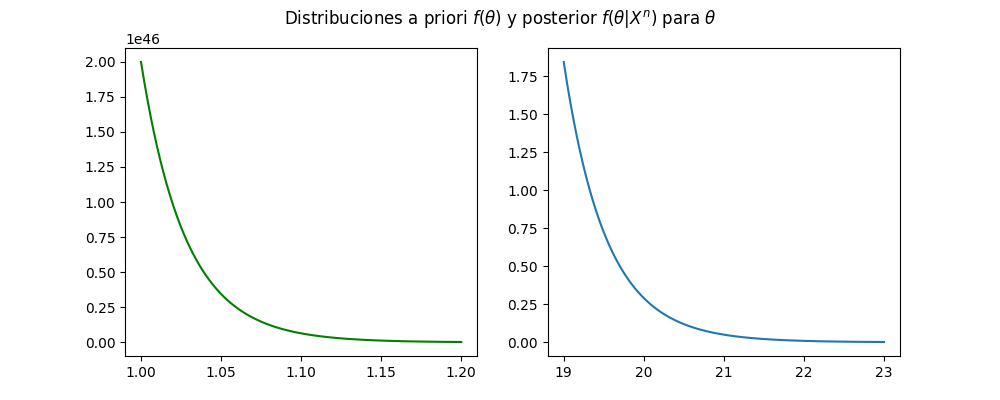
\includegraphics[width = 15 cm]{Figures/distribuciones.png} 
        \caption{Distribución a priori y distribución posterior para $\theta$.}
        \label{Fig. 1.1}
    \end{figure} 
    
\end{solution}


\begin{problem}{2} 
    Si $\mathbf{Y} \sim N_n(\mathbf{X}\theta, \Sigma)$ y $\Sigma$, la matriz de varianzas y covarianzas, conocida (definida positiva); $\mathbf{X}$, la matriz de diseño en la regresión, conocida. Encuentre la posterior $\theta$ usando una $N_p(\mu_0,\Sigma_0 )$ como \textit{a priori}. Encuentre la distribución predictiva de un dato futuro $Y_{n+1}$.
\end{problem}

\begin{solution} 
    Recordemos que la densidad de una variable $\mathbf{X} \sim N_n(\mu, \Sigma)$  (distribución normal n-variada) es 
    \begin{align}
        f(\mathbf{X}|\theta) = (2\pi)^{-n/2}|\Sigma|^{-1/2} \exp  \left \{-\frac{1}{2}\left(\mathbf{X} - \mu\right) ' \Sigma^{-1} \left(\mathbf{X}-\mu\right)  \right \},
    \end{align}
    con $\mathbf{X}, \mu \in \mathbb{R}^{n}$.
    
    Empecemos por encontrar la distribución posterior para $\theta$. Tenemos un modelo normal $n-$variado y se propone una distribución a priori normal $p-$variada. Así la distribución posterior se sigue de 
    \begin{align}
        \pi(\theta|\mathbf{Y}) \propto f(\mathbf{Y}|\theta) \pi (\theta).
    \end{align}
    con $\theta \in \mathbb{R}^{p}$. Luego, el modelo de $\mathbf{Y}$ tiene la siguiente verosimilitud
    \begin{align}
        f(\mathbf{Y}|\theta) = (2\pi)^{-n/2} |\Sigma|^{-1/2} \exp \left \{ -\frac{1}{2}\left(\mathbf{Y}- X\theta\right) ' \Sigma^{-1} \left(\mathbf{Y} - X \theta \right)  \right \}.
        \label{2.03} 
    \end{align}

    Juntando la distribución a priori con (\ref{2.03}) tenemos
    \begin{align*}
        \pi(\theta|\mathbf{Y}) &\propto (2\pi)^{-n/2} |\Sigma|^{-1/2} \exp \left \{ -\frac{1}{2}\left(\mathbf{Y}- X\theta\right) ' \Sigma^{-1} \left(\mathbf{Y} - X \theta \right)  \right \} \cdot \\
        & \:\:\:\:\:\:\:\: (2\pi)^{-p/2}|\Sigma_0| \exp \left \{ -\frac{1}{2} \left(\theta - \mu_0 \right)' \Sigma^{-1}_0 \left(\theta - \mu_0 \right)   \right \} .
    \end{align*}
    Prescindiendo de las constantes
    \begin{align}
        \pi(\theta|\mathbf{Y}) \propto \exp \left \{ -\frac{1}{2} \left[\left(\mathbf{Y} - X\theta \right) ' \Sigma^{-1} \left(\mathbf{Y} - X\theta \right) + \left(\theta - \mu_0\right)' \Sigma^{-1}_0 \left(\theta -\mu_0 \right)    \right]  \right \} .
    \end{align}
    y observamos que es parecido al núcleo de una distribución normal $p-$variada. Para ello buscamos completar la forma cuadrática tal que tengamos un núcleo de la forma
    \begin{align}
        \exp \left \{ -\frac{1}{2} \left(\theta - \mu_n\right)' \Sigma^{-1}_n    \left(\theta  - \mu_n \right)   \right \}.
        \label{2.05} 
    \end{align}
    Consideremos 
    \begin{align*}
        Q = \left(\mathbf{Y} - X\theta \right) ' \Sigma^{-1} \left(\mathbf{Y} - X\theta \right) + \left(\theta - \mu_0\right)' \Sigma^{-1}_0 \left(\theta -\mu_0 \right).
    \end{align*}
    Desarrollando
    \begin{align*}
        Q &= \mathbf{Y}'\Sigma^{-1} \mathbf{Y} - \mathbf{Y}'\Sigma^{-1} X\theta -\theta' X' \Sigma^{-1} \mathbf{Y} + \theta' X' \Sigma^{-1} X\theta + \\
        & \:\:\:\:\:\: +\theta' \Sigma^{-1}_0 \theta - \theta' \Sigma^{-1}_0 \mu_0 - \mu_0' \Sigma^{-1}_0 \theta + \mu_0 '\Sigma^{-1}_0 \mu_0.
    \end{align*}
    Simplificando
    \begin{align}
        Q &= \mathbf{Y}'\Sigma^{-1} \mathbf{Y} - 2\mathbf{Y}'\Sigma^{-1} X\theta + \theta' X' \Sigma^{-1} X\theta + \nonumber\\
        & \:\:\:\:\:\: +\theta' \Sigma^{-1}_0 \theta - 2\theta' \Sigma^{-1}_0 \mu_0 + \mu_0 '\Sigma^{-1}_0 \mu_0.
        \label{2.06}
    \end{align}
    De igual forma para el argumento de (\ref{2.05}) 
    \begin{align}
        \left(\theta - \mu_n\right)'  \Sigma^{-1}_n    \left(\theta  - \mu_n \right) &= \theta' \Sigma_n^{-1}\theta - \theta'\Sigma^{-1}_n\mu_n - \mu_n' \Sigma^{-1}_n  \theta + \mu_n' \Sigma_n^{-1} \mu_n, \nonumber \\ 
        & = \theta' \Sigma_n^{-1}\theta - 2\mu_n' \Sigma^{-1}_n  \theta + \mu_n' \Sigma_n^{-1} \mu_n .
        \label{2.07}
    \end{align}
    Comparando los términos 3 y 4 de (\ref{2.06}) con el primero de (\ref{2.07})
    \begin{align*}
        \theta' \Sigma_n^{-1} \theta = \theta' X' \Sigma^{-1}X\theta + \theta ' \Sigma_0^{-1} \theta = \theta' \left(X'\Sigma^{-1}X + \Sigma_0^{-1}\right) \theta ,
    \end{align*}
    obtenemos la relación
    \begin{align}
        \Sigma_n^{-1} = \Sigma_0^{-1} + X'\Sigma^{-1}X.
        \label{2.08}
    \end{align}
    Luego, comparando los términos 2 y 5 de (\ref{2.06}) con el segundo de (\ref{2.07})
    \begin{align*}
        -2\mu_n' \Sigma_n^{-1} \theta &= -2 \mathbf{Y} \Sigma^{-1}X\theta -2\mu_0\Sigma_0^{-1} \theta, \\
        \mu_n' \Sigma_n^{-1} \theta &=  \left(  \mathbf{Y} \Sigma^{-1}X + \mu_0\Sigma_0^{-1} \right) \theta,
    \end{align*}
    transponiendo se sigue
    \begin{align*}
        \Sigma_n^{-1} \mu_n = X' \Sigma \mathbf{Y} + \Sigma_0^{-1}\mu_0,
    \end{align*}
    lo que concluye que
    \begin{align}
        \mu_n = \Sigma_n \left(X' \Sigma \mathbf{Y} + \Sigma_0^{-1}\mu_0\right),
        \label{2.09}
    \end{align}
    los términos restantes son constantes respecto a $\theta$ por lo que no requiere análisis.

    Así es claro que la distribución posterior es
    \begin{align}
        \theta|\mathbf{Y} \sim N_p (\mu_n, \Sigma_n),
    \end{align}
    con $\mu_n, \Sigma_n$ definidos en (\ref{2.09}) y (\ref{2.08}), respectivamente.

    Por otro lado, para obtener la distribución predictiva para una nueva observación $\mathbf{Y}_{n+1}$ dada las observaciones previas es necesario calcular
    \begin{align*}
        f(\mathbf{Y}_{n+1}| \mathbf{Y}) = \int f(\mathbf{Y}_{n+1}|\theta,\mathbf{Y}) \pi(\theta|\mathbf{Y}) d\theta,
    \end{align*}
    y por independencia de las observaciones 
    \begin{align}
        f(\mathbf{Y}_{n+1}| \mathbf{Y}) = \int f(\mathbf{Y}_{n+1}|\theta) \pi(\theta|\mathbf{Y}) d\theta.
        \label{2.10}
    \end{align}

    Sustituyendo las respectivas densidades en (\ref{2.10})
    \begin{align*}
        f(\mathbf{Y_{n+1}}|\mathbf{Y}) &= \int (2\pi)^{-n/2}|\Sigma|^{-1/2} \exp \left \{ -\frac{1}{2}\left(\mathbf{Y}_{n+1}  - X\theta \right)' \Sigma^{-1} \left(\mathbf{Y}_{n+1}-X\theta  \right) \right \}  \cdot \\
        &\:\:\:\:\:\:\: \cdot (2\pi)^{-p/2}|\Sigma_n|^{-1/2} \exp \left \{ -\frac{1}{2}\left(\theta - \mu_n\right) '\Sigma_n^{-1} \left(\theta - \mu_n  \right)  \right \} d\theta.
    \end{align*}
    Sacando las constante de la integral
    \begin{align*}
        f(\mathbf{Y_{n+1}}|\mathbf{Y}) &= (2\pi)^{-n/2}(2\pi)^{-p/2} |\Sigma|^{-1/2}|\Sigma_n|^{-1/2} \int \exp \left \{ -\frac{1}{2} Q(\theta) \right \} d\theta, 
    \end{align*}
    donde 
    \begin{align}
        Q(\theta) &= \left(\mathbf{Y}_{n+1} - X\theta\right) '\Sigma^{-1}\left(\mathbf{Y}_{n+1} - X\theta \right) + \left(\theta - \mu_n\right) ' \Sigma_n^{-1} \left(\theta - \mu_n\right) ,\nonumber \\
        &= \mathbf{Y}_{n+1}'\Sigma^{-1}\mathbf{Y}_{n+1} - 2\mathbf{Y}_{n+1} \Sigma^{-1}X\theta + \theta'X'\Sigma^{-1}X\theta + \nonumber\\
        &\:\:\:\:\: + \theta'\Sigma_n^{-1}\theta - 2 \mu_n' \Sigma_n^{-1}\theta + \mu_n'\Sigma_n^{-1} \mu_n. 
        \label{2.11}
    \end{align}
    De manera análoga al calculo de la distribución posterior de $\theta$, ahora buscamos tener la forma cuadrática
    \begin{align}
        \left(\theta - \mu_p\right) ' &\Sigma_p^{-1}\left(\theta - \mu_p\right) = \nonumber\\
        &= \theta'\Sigma_p^{-1}\theta -2\mu_p'\Sigma_p^{-1} \theta + \mu_p'\Sigma_p^{-1} \mu_p.
        \label{2.12}
    \end{align}

    Buscamos relaciones de $\mu_p$ y $\Sigma_p$ con los parámetros conocidos. Así, comparando el primer término de (\ref{2.12}) con los términos 3 y 4 de (\ref{2.11}) y además comparando los términos 2 y 5 de (\ref{2.11}) con el segundo término de (\ref{2.12}) obtenemos las relaciones
    \begin{align}
        \Sigma_p^{-1} &= X'\Sigma^{-1}X + \Sigma_n^{-1},
        \label{2.13}
        \\
        \mu_p &= \Sigma_p \left(X'\Sigma^{-1}\mathbf{Y}_{n+1} + \Sigma_n^{-1} \mu_n\right),
        \label{2.14}
    \end{align}
    análogas a las relaciones (\ref{2.08}) y (\ref{2.09}) de la distribución posterior.

    Por tanto, podemos escribir la distribución predictiva como
    \begin{align*}
        f(\mathbf{Y}_{n+1}|\mathbf{Y}) &= (2\pi)^{-n/2}(2\pi)^{-p/2}|\Sigma|^{-1/2}|\Sigma_n |^{-1/2} \cdot \\ & \:\:\:\:\:\: \cdot \int \exp \left \{-\frac{1}{2} \left[ \left(\theta - \mu_p\right) '\Sigma_p^{-1} \left(\theta - \mu_p\right) + \mathbf{Y}_{n+1}'\Sigma^{-1}\mathbf{Y}_{n+1} + \mu_n'\Sigma_n^{-1}\mu_n \right] \right  \} d\theta .
    \end{align*}
    Reordenando 
    \begin{align*}
        f(\mathbf{Y}_{n+1}|\mathbf{Y}) &= (2\pi)^{-n/2}|\Sigma|^{-1/2}|\Sigma_n |^{-1/2}|\Sigma_p|^{1/2}\exp \left \{  -\frac{1}{2} \left(\mathbf{Y}_{n+1}' \Sigma^{-1} \mathbf{Y}_{n+1}+ \mu_n' \Sigma_n^{-1}\mu_n \right)   \right \}  \cdot \\
        &\:\:\:\:\:\:\: \cdot \int (2\pi)^{-p/2} |\Sigma_p|^{-p/2}\exp \left \{ -\frac{1}{2}\left(\theta - \mu_p\right) ' \Sigma_p^{-1}\left(\theta - \mu_p\right) \right \}d\theta .
    \end{align*}
    Vemos que la integral corresponde a la integral de una distribución normal $p-$variada con media $\mu_p$ y matriz de covarianzas $\Sigma_p$, por tanto integra uno. Finalmente
    \begin{align}
        f(\mathbf{Y}_{n+1}|\mathbf{Y}) &= (2\pi)^{-n/2}|\Sigma|^{-1/2}|\Sigma_n |^{-1/2}|\Sigma_p|^{1/2}\exp \left \{  -\frac{1}{2} \left(\mathbf{Y}_{n+1}' \Sigma^{-1} \mathbf{Y}_{n+1}+ \mu_n' \Sigma_n^{-1}\mu_n \right)   \right \},
        \label{2.15}
    \end{align}
    que es la función de densidad de la distribución predictiva.
\end{solution}



\begin{problem}{3} 
    Sea el modelo de crecimiento logístico $\frac{dX}{dt} = \theta_1 X \left( \theta_2 - X  \right)$ con $X(0) = X_0$. Suponga que tenemos observaciones $y_i$ para $X(t_i), t_1 < t_2 < \cdots < t_n$, con ruido gaussiano aditivo independiente, esto es
    \begin{align*}
        y_i = X(t_i) + \epsilon_i; \:\:\:\:\: \epsilon_i \sim N(0,\sigma), \:\:\: i = 1,2,\cdots,n.
    \end{align*} 
    Simule datos con $X(0) = 100$, $\theta_1 =$ 0.001, $\theta_2 = $ 1000, $\sigma = 30$ , $n= 26$ equiespaciados en $t \in [0,10]$. Haga inferencia bayesiana para los parámetro $\theta_1, \theta_2$. Utilice a priories Gamma, centradas en los valores verdaderos. ¿Qué puede decir de la tasa de crecimiento que es $\lambda = \theta_1\theta_2$ ?
\end{problem}

\begin{solution} 
    Para este ejercicio se tiene se implemento numéricamente la ecuación diferencial correspondiente al crecimiento logístico. Luego, simulamos 26 datos en un arreglo equiespaciado del tiempo con un ruido gaussiano tal como se pide en el enunciado. Podemos ver los datos graficados en la Fig \ref{Fig. 3.01}

    \begin{figure}[H] 
        \centering 
        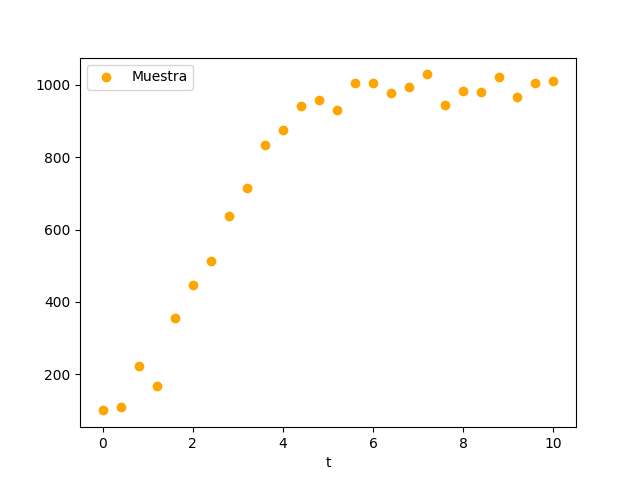
\includegraphics[width = 10 cm]{Figures/Muestra.png} 
        \caption{Simulación de datos de crecimiento logístico.}
        \label{Fig. 3.01}
    \end{figure}    

    La distribución posterior es
    \begin{align}
        \pi(\theta_1,\theta_2|\mathbf{y}) \propto \mathcal{L}(\theta_1,\theta_2)  \pi(\theta_1,\theta_2),
        \label{3.01}
    \end{align}

    donde la verosimilitud se obtiene del modelo gaussiano. Así
    \begin{align}
        \mathcal{L}(\theta_1,\theta_2) &= \prod_{i = 1}^{n} \frac{1}{\sqrt{2\pi\sigma^2}} \exp \left \{ -\frac{1}{2\sigma^2} \left(y_i - F_{\theta}(t_i)\right) ^2   \right \}, \nonumber\\
        &= \left(\frac{1}{2\pi\sigma^2}\right)^{n/2} \exp \left \{  -\frac{1}{2\sigma^2} \sum_{i = 1}^{n}\left(y_i - F_{\theta}(t_i)\right)^2 \right \}.
        \label{3.02}
    \end{align}
    
    Elegimos las distribuciones a priori gammas independientes
    \begin{align*}
        \theta_1 \sim Gamma\left(\alpha_0, \frac{\text{0.001}}{\alpha_0} \right) ,\\
        \theta_2 \sim Gamma\left(\beta_0, \frac{1000}{\beta_0}\right) ,
    \end{align*}
    con $\alpha_0 = \beta_0 = 1000$. Así
    \begin{align}
        \pi(\theta_1,\theta_2) = \left(\frac{\text{0.001}}{\alpha_0}\right) ^{\alpha_0} \frac{\theta_1^{\alpha_0-1}\exp \left \{ -\text{0.001}\alpha_0 /\theta_1\right \} }{\Gamma(\alpha_0)}\cdot \left(\frac{\text{1000}}{\beta_0}\right) ^{\beta_0} \frac{\theta_2^{\beta_0-1}\exp \left \{ -\text{1000}\beta_0 /\theta_2\right \} }{\Gamma(\beta_0)}.
        \label{3.03}
    \end{align}

    Las distribuciones a priori se dan en la Fig \ref{Fig. 3.02} con los parámetros anteriormente descritos.
    \begin{figure}[H] 
        \centering 
        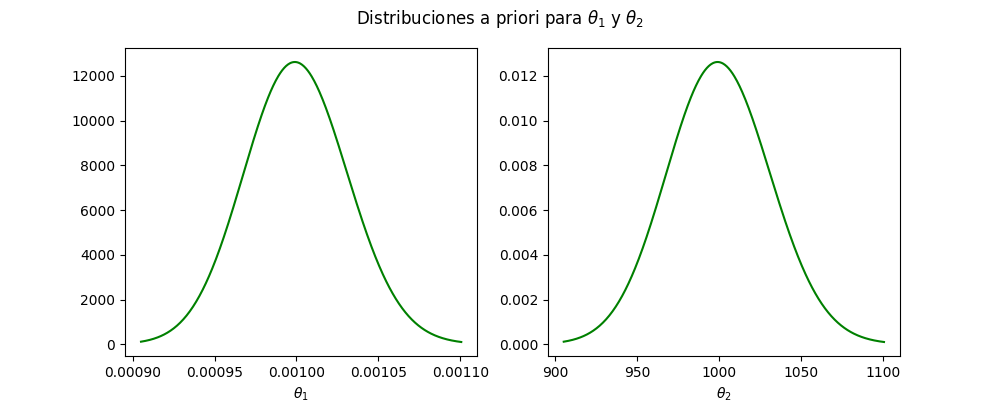
\includegraphics[width = 15cm]{Figures/Apriori.png} 
        \caption{Distribuciones a priori para $\theta_1$ y $\theta_2$.}
        \label{Fig. 3.02}
    \end{figure} 

    Sustituyendo (\ref{3.02}) y (\ref{3.03}) en (\ref{3.01}) tenemos la distribución objetivo. La cual por medio de métodos Monte Carlo podemos simular de dicha distribución. Con MCMC simulamos una cadena de tamaño $T=$100000 tomamos las marginales de la posterior para cada parámetro las cuales vemos en la Fig \ref{Fig. 3.03} y en la Fig \ref{Fig. 3.04}.

    \begin{figure}[H] 
        \centering 
        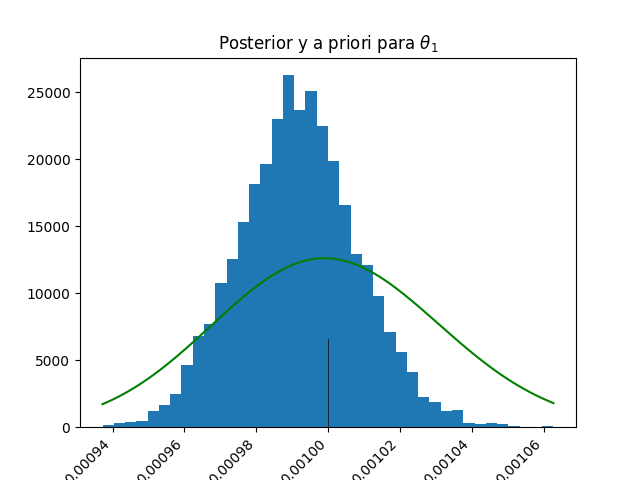
\includegraphics[width = 10 cm]{Figures/Post_theta_1.png} 
        \caption{Distribución marginal posterior para $\theta_1$ (azul) y distribución a priori (verde) con parámetro verdadero (negro).}
        \label{Fig. 3.03}
    \end{figure} 

    \begin{figure}[H] 
        \centering 
        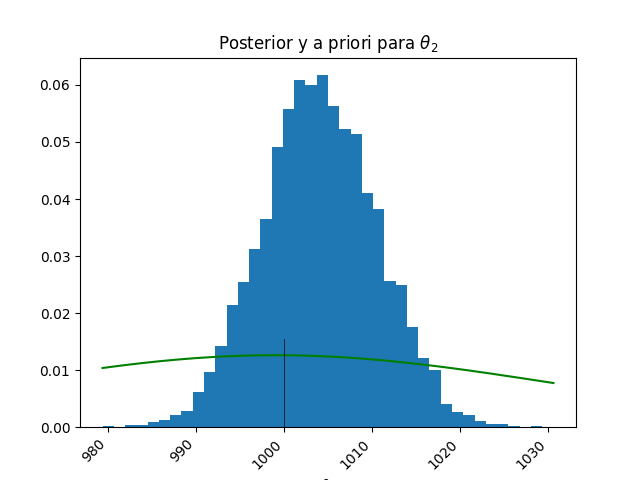
\includegraphics[width = 10 cm]{Figures/Post_theta_2.png} 
        \caption{Distribución marginal posterior para $\theta_2$ (azul) y distribución a priori (verde) con parámetro verdadero (negro).}
        \label{Fig. 3.04}
    \end{figure} 

    De igual forma, para la tasa de crecimiento $\lambda$ obtenemos el histograma posterior obtenido simplemente de tomar el producto de cada marginal posterior, graficado en la Fig \ref{Fig. 3.05}.
    \begin{figure}[H] 
        \centering 
        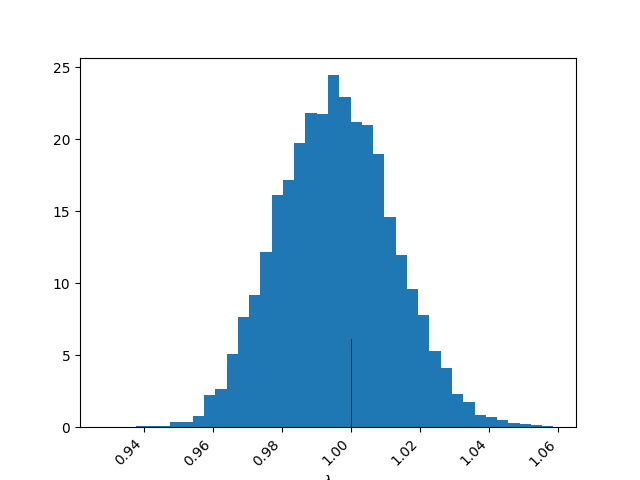
\includegraphics[width = 10 cm]{Figures/Lambda.png} 
        \caption{Posterior para parámetro de tasa de crecimiento $\lambda$.}
        \label{Fig. 3.05}
    \end{figure} 

    Finalmente, graficamos la distribución predictiva de la cadena tomando submuestreos de la cadena fruto de MCMC y tomando la media en cada submuestreo para considerar la trayectoria generada por el forward map en la Fig \ref{Fig. 3.06}.
    \begin{figure}[H] 
        \centering 
        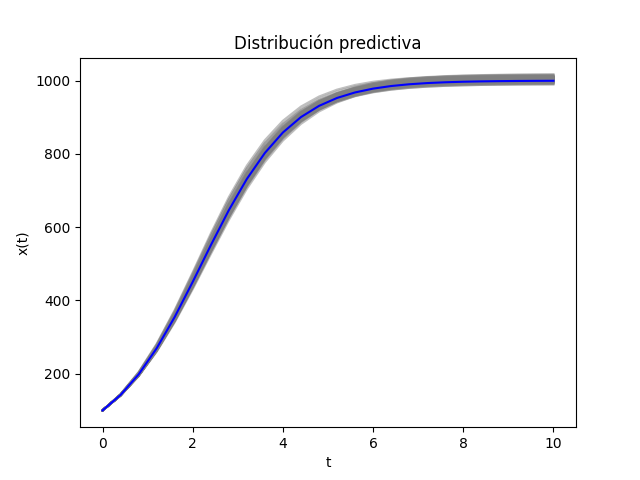
\includegraphics[width = 10 cm ]{Figures/Predictiva.png} 
        \caption{Distribución predictiva para crecimiento logístico (gris) y la trayectoria real simulada (azul).}
        \label{Fig. 3.06}
    \end{figure} 

    Notamos que dicha distribución predictiva ajusta satisfactoriamente a la trayectoria simulada con los parámetros reales.
    
\end{solution}



% \begin{thebibliography}{9}

%     \bibitem{Casella}
%     Robert, C. P., Casella, G., and Casella, G. (1999). Monte Carlo statistical methods (Vol. 2). New York: Springer.

%     \bibitem{Wasserman}
%     Wasserman, L. (2004). All of statistics: a concise course in statistical inference (p. 413). New York: Springer.
    
% \end{thebibliography}
      

\end{document}